\subsection{Princip inkluze a exkluze}
\label{ssec:princip-inkluze-a-exkluze}

Další základní úlohou, která se objevuje napříč diskrétní matematikou, je
problém velikosti sjednocení množin.

Velikost průniku se dá spočítat snadno. Člověk se zkrátka podívá, které prvky
leží v každé množině, a spočítá je. Vlastně stačí vzít tu nejmenší množinu a
započítat jen ty prvky, které leží i ve všech ostatních.

Se sjednocením je to však těžší, neboť některé prvky mohou ležet v jedné
množině, ve všech množinách nebo v jakémkoli počtu množin mezi těmito extrémy.
Měl-li by člověk počítat velikost sjednocení manuálně, musel by množiny
procházet jednu po druhé a navíc si u každého prvku pamatovat, zda ho už
započetl, či ještě ne. Tento způsob je sice algoritmicky přímočarý, ale
neefektivní i z~hlediska výpočetního. Navíc často není ani použitelný, protože
se může stát, že znám jen velikosti jednotlivých množin, ale ne přesný výčet 
jejich prvků. Lepší způsob, který si teď ukážeme a vysvětlíme, počítá, možná i
trochu překvapivě, velikost sjednocení vlastně jako součet přes všechny možné
průniky.

Nejprve jakýsi \uv{motivační} příklad. Jeho praktické využití je za účelem
zachování jednoduchosti pravdaže poněkud omezené.

\begin{example}
 \label{exam:inkluze-exkluze}
 Na Gymnáziu Growth Severní Obec je možné se učit třem cizím jazykům -- němčině,
 španělštině a francouzštině. Německy se učí 30 studentů, španělsky 25 studentů
 a 2 velmi nešťastné osoby se učí francouzsky. Přitom, mezi němčináři jsou 4
 španělštináři a jeden bageťák. Exkluzivně románským jazykům neholduje nikdo.
 Jeden no-lifer se ale dokonce učí všem třem jazykům naráz.

 Kolik celkem studentů se učí aspoň jednomu cizímu jazyku?
\end{example}

Můžete si zkusit úlohu vyřešit manuálně. Chvíli vám to zabere a na konci navíc
zjistíte, že jste vynalezli tzv. \emph{princip inkluze a exkluze}, což je
honosný název pro vzoreček, který říká, že velikost sjednocení množin dostanu
tak, že sečtu velikosti všech průniků lichého počtu množin a odečtu velikosti
průniků sudého počtu množin.

Protože vám předchozí věta vůbec nic neřekla, ukážeme si nejprve na třech
množinách (a pomocí obrázků), jak \emph{princip inkluze a exkluze} funguje.

Uvažujme tři množiny $\clr{A},\clb{B}$ a $\clg{C}$ s neprázdným průnikem, tedy
$\clr{A} \cap \clb{B} \cap \clg{C} \neq \emptyset$. Nakreslenou vidíte tuto
situaci na
\hyperref[fig:inkluze-exkluze-1]{obrázku~\ref*{fig:inkluze-exkluze-1}}.

\begin{figure}[h]
 \centering
 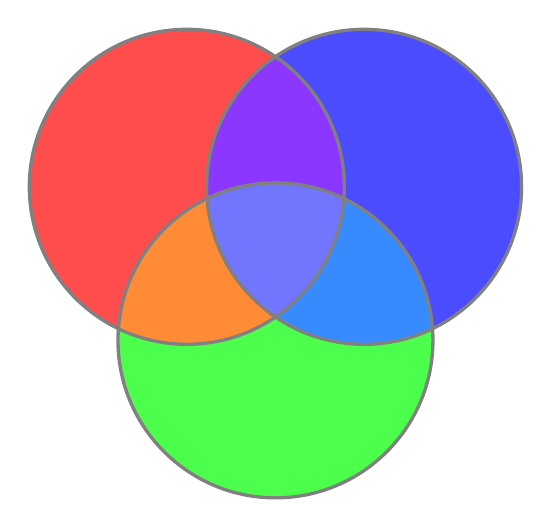
\begin{tikzpicture}
  \begin{scope}[blend group=soft light]
   \fill[blue!70!white] (30:1.3) circle (2cm);
   \fill[red!70!white] (150:1.3) circle (2cm);
   \fill[green!70!white] (270:1.3) circle (2cm);
  \end{scope}
  \draw[gray,very thick] (30:1.3) circle (2cm);
  \draw[gray,very thick] (150:1.3) circle (2cm);
  \draw[gray,very thick] (270:1.3) circle (2cm);
 \end{tikzpicture}
 \caption{Množiny $\clr{A}, \clb{B}, \clg{C}$ s neprázdným průnikem.}
 \label{fig:inkluze-exkluze-1}
\end{figure}

Budeme nyní počítat velikost sjednocení $\clr{A} \cup \clb{B} \cup \clg{C}$.

Za předpokladu, že by množiny byly disjunktní, stačilo by zkrátka sečíst
velikosti jednotlivých množin. V této situaci však započteme některé prvky
vícekrát. Stane se to proto, že když sečtu třeba $\# \clr{A} + \# \clb{B}$, tak
prvky, které leží i v $\clr{A}$ i v $\clb{B}$ (tedy ty v průniku
\textcolor[HTML]{7f33e8}{$A \cap B$}) započtu dvakrát. Na
\hyperref[fig:inkluze-exkluze-2]{obrázku níže} vidíte, kolikrát započteme který
\uv{díl} svého Vennova diagramu.

\begin{figure}[h]
 \centering
 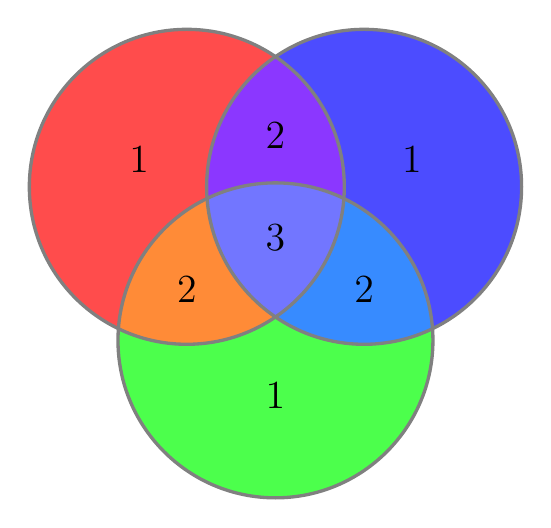
\begin{tikzpicture}
  \begin{scope}[blend group=soft light]
   \fill[blue!70!white] (30:1.3) circle (2cm);
   \fill[red!70!white] (150:1.3) circle (2cm);
   \fill[green!70!white] (270:1.3) circle (2cm);
  \end{scope}
  \draw[gray,very thick] (30:1.3) circle (2cm);
  \draw[gray,very thick] (150:1.3) circle (2cm);
  \draw[gray,very thick] (270:1.3) circle (2cm);
  
  \foreach \angle in {30,150,270} {
   \node at (\angle:2) {\Large $1$};
  }
  \foreach \angle in {90,210,330} {
   \node at (\angle:1.3) {\Large $2$};
  }
  \node at (0,0) {\Large $3$};
 \end{tikzpicture}
 \caption{Znázornění součtu $\# \clr{A} + \# \clb{B} + \# \clg{C}$.}
 \label{fig:inkluze-exkluze-2}
\end{figure}

Jak můžete vyčíst z \hyperref[fig:inkluze-exkluze-2]{obrázku}, některé průniky
jsme započítali mockrát. Černá čísla značí, kolikrát jsme každý kousek
sjednocení započetli, když jsme sečetli $\# \clr{A} + \# \clb{B} + \# \clg{C}$.
Například jsme tedy započetli každý prvek ležící v průniku
$\textcolor[HTML]{e78033}{A \cap C}$ dvakrát a každý prvek v průniku
$\textcolor[HTML]{6a6ee9}{A \cap B \cap C}$ dokonce třikrát.

Abychom situaci napravili, a započetli průnik každého páru množin jen jednou,
odečteme od součtu $\# \clr{A} + \# \clb{B} + \# \clg{C}$ velikosti všech
průniků dvou množin. Odpovídající diagram vidíte
\hyperref[fig:inkluze-exkluze-3]{níže}.

\begin{figure}[h]
 \centering
 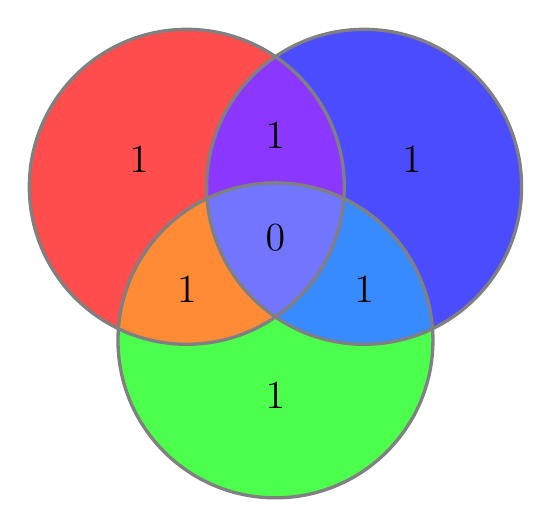
\begin{tikzpicture}
  \begin{scope}[blend group=soft light]
   \fill[blue!70!white] (30:1.3) circle (2cm);
   \fill[red!70!white] (150:1.3) circle (2cm);
   \fill[green!70!white] (270:1.3) circle (2cm);
  \end{scope}
  \draw[gray,very thick] (30:1.3) circle (2cm);
  \draw[gray,very thick] (150:1.3) circle (2cm);
  \draw[gray,very thick] (270:1.3) circle (2cm);
  
  \foreach \angle in {30,150,270} {
   \node at (\angle:2) {\Large $1$};
  }
  \foreach \angle in {90,210,330} {
   \node at (\angle:1.3) {\Large $1$};
  }
  \node at (0,0) {\Large $0$};
 \end{tikzpicture}
 \caption{Znázornění výrazu $\# \clr{A} + \# \clb{B} + \# \clg{C} - \#
 \textcolor[HTML]{7f33e8}{A \cap B} - \# \textcolor[HTML]{e78033}{A \cap C} - \#
 \textcolor[HTML]{3a87ef}{B \cap C}$.}
 \label{fig:inkluze-exkluze-3}
\end{figure}

Ovšem, nyní jsme zase odečetli třikrát průnik $\textcolor[HTML]{6a6ee9}{A \cap B
\cap C}$, protože každý prvek v $\textcolor[HTML]{6a6ee9}{A \cap B \cap C}$ leží
zároveň v $\textcolor[HTML]{7f33e8}{A \cap B}$, v $\textcolor[HTML]{e78033}{A
\cap C}$ i v $\textcolor[HTML]{3a87ef}{B \cap C}$, a ty jsme všechny odečetli.
Tedy nám z průniku $\textcolor[HTML]{6a6ee9}{A \cap B \cap C}$ žádné prvky
nezůstaly. Situaci napravíme tím, že jeho velikost přičteme zpátky. Celkově
dostaneme pro velikost sjednocení $\# A \cup B \cup C$ vzorec
\[
 \# A \cup B \cup C = \# \clr{A} + \# \clb{B} + \# \clg{C} - \#
 \textcolor[HTML]{7f33e8}{A \cap B} - \# \textcolor[HTML]{e78033}{A \cap C} - \#
 \textcolor[HTML]{3a87ef}{B \cap C} + \# \textcolor[HTML]{6a6ee9}{A \cap B \cap
 C}.
\]
Finální znázornění vidíte na
\hyperref[fig:inkluze-exkluze-4]{obrázku~\ref*{fig:inkluze-exkluze-4}}.

\begin{figure}[h]
 \centering
 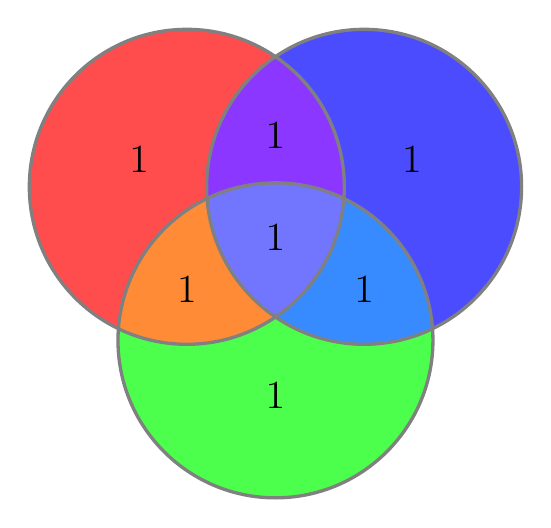
\begin{tikzpicture}
  \begin{scope}[blend group=soft light]
   \fill[blue!70!white] (30:1.3) circle (2cm);
   \fill[red!70!white] (150:1.3) circle (2cm);
   \fill[green!70!white] (270:1.3) circle (2cm);
  \end{scope}
  \draw[gray,very thick] (30:1.3) circle (2cm);
  \draw[gray,very thick] (150:1.3) circle (2cm);
  \draw[gray,very thick] (270:1.3) circle (2cm);
  
  \foreach \angle in {30,150,270} {
   \node at (\angle:2) {\Large $1$};
  }
  \foreach \angle in {90,210,330} {
   \node at (\angle:1.3) {\Large $1$};
  }
  \node at (0,0) {\Large $1$};
 \end{tikzpicture}
 \caption{Velikost sjednocení $\# A \cup B \cup C$ podle principu inkluze a
 exkluze.}
 \label{fig:inkluze-exkluze-4}
\end{figure}

Formální znění principu inkluze a exkluze dí, že tento postup funguje zcela
obecně, tedy že pokud průniky sudého počtu množin odečítám a lichého počtu
přičítám, dostanu tím velikost sjednocení.

Ještě předtím, než ho uvedeme a dokážeme, si ale určíme počet studentů
z~\hyperref[exam:inkluze-exkluze]{úvodního příkladu}. Množiny němčinářů,
španělštinářů a francouzštinářů označíme po řadě $N$, $\check{S}$ a $\check{Z}$
(jako \textbf{ž}abožrout). Ze zadání víme, že $\# N = 30, \# \check{S} = 25$ a
$\# \check{Z} = 2$. Dále víme, že $\# N \cap \check{S} = 4$, protože mezi
němčináři jsou čtyři španělštináři; podobně $\# N \cap \check{Z} = 1$ a $\#
\check{S} \cap \check{Z} = 0$. Konečně, $\# N  \cap \check{S} \cap \check{Z} =
1$. Podle principu inkluze a exkluze máme
\begin{align*}
 \# N \cup \check{S} \cup \check{Z} &= \# N + \# \check{S} + \# \check{Z} - \# N
  \cap \check{S} - \# N  \cap \check{Z} - \# \check{S} \cap \check{Z} + \# N
  \cap \check{S}  \cap \check{Z}\\
 &= 30 + 25 + 2 - 4 - 1 - 0 + 1 = 53.
\end{align*}
Celkem se tedy na Gymnáziu Growth Severní Obec učí 53 studentů cizím jazykům.

Posledním krokem, který zbývá, je umět princip inkluze a exkluze nějak rozumně
zapsat. Tohle je asi první situace, na kterou jsme narazili, kdy bez rozumného
zápisu daného tvrzení bychom se ze symbolů doslova zbláznili (hlavně v jeho
důkazu). Natvrdo napsaný říká princip inkluze a exkluze, že
\begin{align*}
 \# \bigcup_{i=1}^{n} A_i &= \# A_1 + \# A_2 + \cdots + \# A_n\\
 &- \# A_1 \cap A_2 - \# A_1 \cap A_3 - \cdots - \# A_1 \cap A_n - \# A_2
 \cap A_3 - \cdots - \# A_{n-1} \cap A_n\\
 &+ \# A_1 \cap A_2 \cap A_3 + \cdots + \# A_{n-2} \cap A_{n-1} \cap A_n +
 \cdots + (-1)^{n-1} \bigcap_{i=1}^{n} A_i.
\end{align*}
Jak sami vidíte, z tohoto zápisu je sotva (pokud vůbec) poznat, čemu se vlastně
velikost sjednocení $\bigcup_{i=1}^{n} A_i$ rovná. Musíme tento zápis
zjednodušit. Nejprve, pro každou $I \subseteq \{1,\ldots,n\}$ znamená zápis
\[
 \bigcap_{i \in I}^{} A_i
\]
průnik přesně těch množin $A_i$, jejichž indexy leží v množině $I$. Je-li tedy
např. $I = \{1,4,5\}$, pak
\[
 \bigcap_{i  \in I}^{} A_i = A_1 \cap A_4 \cap A_5.
\]
Pro extrémní případ $I = \emptyset$ dodefinujeme $\bigcap_{i \in  I}^{}A_i
\coloneqq \emptyset$, tedy prázdný průnik je prázdná množina.

Dále si rozmyslíme jednoduchý způsob, jak zapsat znaménko u každého z průniků.
Víme, že průnik sudého počtu množin má záporné znaménko a průnik lichého počtu
má kladné. Ještě jinak, když $\# I$ je sudé číslo, pak $\bigcap_{i \in  I}^{}
A_i$ musí dostat záporné znaménko, a když $\# I$ je liché číslo, tak kladné. V
matematice se pro tyto účely obvykle používá $(-1)^{k}$ pro přirozené číslo $k
\in \N$, protože $(-1)^{k}=1$, když $k$ je sudé, a $(-1)^{k} = -1$, když $k$ je
liché. To ale znamená, že výraz $\# \bigcap_{i \in  I}^{} A_i$ musí být
vynásobený číslem $(-1)^{\# I-1}$.

Už jsme skoro hotovi. Pro vyjádření $\# \bigcup_{i=1}^{n} A_i$ pomocí průniků
musíme sečíst velikosti všech průniků $k$ různých množin pro $k$ od $1$ až do
$n$ se správným znaménkem. Čili, musíme sčítat všechny výrazy $(-1)^{\# I - 1}\#
\bigcap_{i \in  I}^{} A_i$ pro všechny podmnožiny $I \subseteq \{1,\ldots,n\}$.

Předchozí diskuse nám umožňuje zapsat princip inkluze a exkluze jako rovnost
\[
 \# \bigcup_{i=1}^{n} A_i = \sum_{I \subseteq \{1,\ldots,n\}}^{} (-1)^{\# I - 1}
 \# \bigcap_{i \in  I}^{} A_i,
\]
kde symbol $\sum_{I \subseteq \{1,\ldots,n\}}^{}$ značí součet přes všechny
\textbf{podmnožiny} množiny $\{1,\ldots,n\}$.

Ještě jednou tedy princip inkluze a exkluze formulujeme jako větu.

\begin{theorem}[Princip inkluze a exkluze]
 \label{thm:princip-inkluze-a-exkluze}
 Ať $A_1,A_2,\ldots,A_n$ jsou množiny. Pak platí rovnost
 \begin{equation*}
  \label{eq:inkluze-exkluze}
  \tag{$\triangle$}
  \# \bigcup_{i=1}^{n} A_i = \sum_{I \subseteq \{1,\ldots,n\}}^{} (-1)^{\# I -
  1} \# \bigcap_{i \in  I}^{} A_i.
 \end{equation*}
\end{theorem}
\begin{proof}
 Důkaz povedeme indukcí podle $n$.

 Když $n = 1$, pak na levé straně rovnosti \eqref{eq:inkluze-exkluze} máme
 \[
  \# \bigcup_{i=1}^{1} A_i = \# A_1
 \]
 a na pravé straně
 \begin{align*}
  \sum_{I \subseteq \{1\}}^{} (-1)^{\# I - 1} \# \bigcap_{i \in  I}^{} A_i &=
  (-1)^{\#\emptyset-1} \# \bigcap_{i  \in \emptyset}^{} A_i + (-1)^{\#\{1\}-1}
  \# \bigcap_{i  \in \{1\}}^{} A_i\\
  &= (-1)^{-1} \cdot 0 + (-1)^{0} \cdot \# A_1 = \# A_1,
 \end{align*}
 protože jediné podmnožiny $\{1\}$ jsou $\emptyset$ a $\{1\}$. Čili pro $n = 1$ 
 rovnost \eqref{eq:inkluze-exkluze} platí.

 Předpokládejme nyní, že rovnost platí pro všechna čísla menší než $n$ a
 dokazujme rovnost pro $n$. Sjednocení na levé straně \eqref{eq:inkluze-exkluze}
 můžeme napsat jako
 \[
  \bigcup_{i=1}^{n} A_i = \clr{\bigcup_{i=1}^{n-1} A_i} \cup \clb{A_n}.
 \]
 Označíme si $\clr{B_1} \coloneqq \clr{\bigcup_{i=1}^{n-1} A_i}$ a $\clb{B_2}
 \coloneqq \clb{A_n}$. Podle principu inkluze a exkluze pro 2 množiny (ten
 můžeme použít z indukčního předpokladu) máme
 \[
  \# \clr{B_1} \cup \clb{B_2} = \# \clr{B_1} + \# \clb{B_2} - \# \clr{B_1} \cap
  \clb{B_2}.
 \]
 Přepsání zpět do množin $A_i$ nám dá
 \[
  \# \bigcup_{i=1}^{n} A_i= \# \clr{\bigcup_{i=1}^{n-1} A_i} \cup \clb{A_n} = \#
  \clr{\bigcup_{i=1}^{n-1} A_i} + \# \clb{A_n} - \#
  \left(\clr{\bigcup_{i=1}^{n-1} A_i} \cap \clb{A_n}\right).
 \]
 Nejprve si uvědomíme, že
 \[
  \left(\clr{\bigcup_{i=1}^{n-1} A_i}\right) \cap \clb{A_n} =
  \bigcup_{i=1}^{n-1} (\clr{A_i} \cap \clb{A_n}),
 \]
 tedy, že je to samé sjednotit množiny $\clr{A_i}$ a pak je proniknout s
 množinou $\clb{A_n}$ jako nejprve proniknout každou množinu $\clr{A_i}$ s
 množinou $\clb{A_n}$ a pak všechny ty průniky sjednotit.

 Teď můžeme (opět z indukčního předpokladu) použít princip inkluze a exkluze na
 sjednocení $\bigcup_{i=1}^{n-1} \clr{A_i}$ a zároveň na $\bigcup_{i=1}^{n-1}
 (\clr{A_i} \cap \clb{A_n})$.

 Dostaneme
 \[
  \# \bigcup_{i=1}^{n-1} \clr{A_i} = \sum_{I \subseteq \{1,\ldots,n-1\}}
  (-1)^{\# I - 1} \# \bigcap_{i \in  I}^{} \clr{A_i}
 \]
 a
 \[
  \# \bigcup_{i=1}^{n-1} (\clr{A_i} \cap \clb{A_n}) = \sum_{I \subseteq
  \{1,\ldots,n-1\}}^{} (-1)^{\# I - 1} \# \bigcap_{i \in  I}^{} (\clr{A_i} \cap
  \clb{A_n}). 
 \]
 Na jedné straně tedy máme vyjádření
 \begin{equation}
  \label{eq:ink-exk-1}
  \begin{split}
   \# \bigcup_{i=1}^{n} A_i &= \sum_{I \subseteq \{1,\ldots,n-1\}}^{} (-1)^{\# I -
   1} \# \bigcap_{i \in  I}^{} \clr{A_i} + \# \clb{A_n}\\
   &- \sum_{I \subseteq \{1,\ldots,n-1\}}^{} (-1)^{\# I - 1} \# \bigcap_{i \in
   I}^{} (\clr{A_i} \cap \clb{A_n}).
  \end{split}
 \end{equation}
 Na druhé straně potřebujeme dokázat (\textbf{ještě to nevíme!}), že
 \begin{equation}
  \label{eq:ink-exk-2}
  \# \bigcup_{i=1}^{n} A_i  \overset{?}{=} \sum_{I \subseteq \{1,\ldots,n\}}^{}
  (-1)^{\# I - 1} \# \bigcap_{i \in  I}^{} A_i.
 \end{equation}
 Porovnáváme tedy součty na pravých stranách rovností \eqref{eq:ink-exk-1} a
 \eqref{eq:ink-exk-2}. Jediný rozumný způsob, jak to udělat, je podívat se, že
 každý sčítanec v~\eqref{eq:ink-exk-2} je rovněž sčítancem v
 \eqref{eq:ink-exk-1}.

 Rozlišíme dva případy podle toho, zda podmnožina $I$ obsahuje $n$, či ne.
 \begin{enumerate}[label=(\alph*)]
  \item Ať nejprve $n \notin I$. Pak v sumě \eqref{eq:ink-exk-2} je sčítanec
   \[
    (-1)^{\# I-1} \# \bigcap_{i \in  I}^{} A_i,
   \]
   kde ten průnik neobsahuje $A_n$, protože $n \notin I$. Jenže pak je $I
   \subseteq \{1,\ldots,n-1\}$, a tedy i součet \eqref{eq:ink-exk-1} obsahuje
   ten samý sčítanec (v té úplně první sumě nahoře) se stejným znaménkem.
  \item Teď předpokládáme, že $n \in I$. Musíme rozlišit zase dva případy (xD).
   \begin{enumerate}[label=(\greek*)]
    \item $I = \{n\}$. Pak součet \eqref{eq:ink-exk-2} obsahuje sčítanec
     \[
      (-1)^{\#\{n\}-1} \# \bigcap_{i \in \{n\}}^{} A_i = \# A_n,
     \]
     který je ale i v součtu \eqref{eq:ink-exk-1} (mezi těmi dvěma sumami).
    \item $I$ obsahuje $n$ a $\# I \geq 2$. V tomto případě máme v součtu
     \eqref{eq:ink-exk-2} sčítanec
     \[
      (-1)^{\# I - 1} \# \bigcap_{i \in I}^{} A_i,
     \]
     jejž si však můžeme přepsat jako
     \begin{align*}
      (-1)^{\# I - 1} \# \bigcap_{i \in I}^{} A_i &= (-1)^{\# I - 1} \#
      \left(\bigcap_{i \in  I \setminus \{n\}}^{} \clr{A_i}\right) \cap
      \clb{A_n}\\
      &= (-1)^{\# I - 1} \# \bigcap_{i  \in I \setminus \{n\}}^{} (\clr{A_i}
      \cap \clb{A_n}),
     \end{align*}
     jelikož předpokládáme, že $n \in I$. Protože $I \setminus \{n\} \subseteq
     \{1,\ldots,n-1\}$, je v součtu \eqref{eq:ink-exk-1} (v té sumě dole)
     sčítanec
     \[
     (-1)^{\#(I \setminus \{n\}) - 1} \# \bigcap_{i  \in I \setminus \{n\}}^{}
     (\clr{A_i} \cap \clb{A_n}),
     \]
     což je v podstatě tentýž, až na znaménko. To však není problém, neboť si
     můžete všimnout, že v součtu \eqref{eq:ink-exk-1} tu druhou sumu obsahující
     všechny průniky s množinou $\clb{A_n}$ odečítám. Tedy, odpovídající
     sčítanec má ve skutečnosti znaménko $-(-1)^{\# (I \setminus \{n\})-1} =
     (-1)^{\# I - 1}$.
   \end{enumerate}
 \end{enumerate}
 Tím jsme ověřili, že součet ve vyjádření \eqref{eq:ink-exk-1} obsahuje přesně
 tytéž sčítance jako součet ve vyjádření \eqref{eq:ink-exk-2}, a tudíž se jedná
 o stejný součet. Tím je podle principu matematické indukce důkaz dokončen.
\end{proof}

Nakonec se podíváme, že
\hyperref[thm:princip-inkluze-a-exkluze]{věta~\ref*{thm:princip-inkluze-a-exkluze}}
souhlasí plně s naší intuicí v již prozkoumaném případě tří množin s neprázdným
průnikem.

\begin{example}
 Uvažme množiny $A_1,A_2,A_3$ takové, že $A_1 \cap A_2 \cap A_3 \neq \emptyset$.
 Podle \hyperref[thm:princip-inkluze-a-exkluze]{principu inkluze a exkluze}
 počítáme
 \[
  \# A_1 \cup A_2 \cup A_3 = \sum_{I \subseteq \{1,2,3\}}^{} (-1)^{\#I - 1}\#
  \bigcap_{i \in  I}^{} A_i.
 \]
\end{example}
